\documentclass{standalone}
\usepackage{tikz}
\usetikzlibrary{patterns, positioning}


\begin{document}
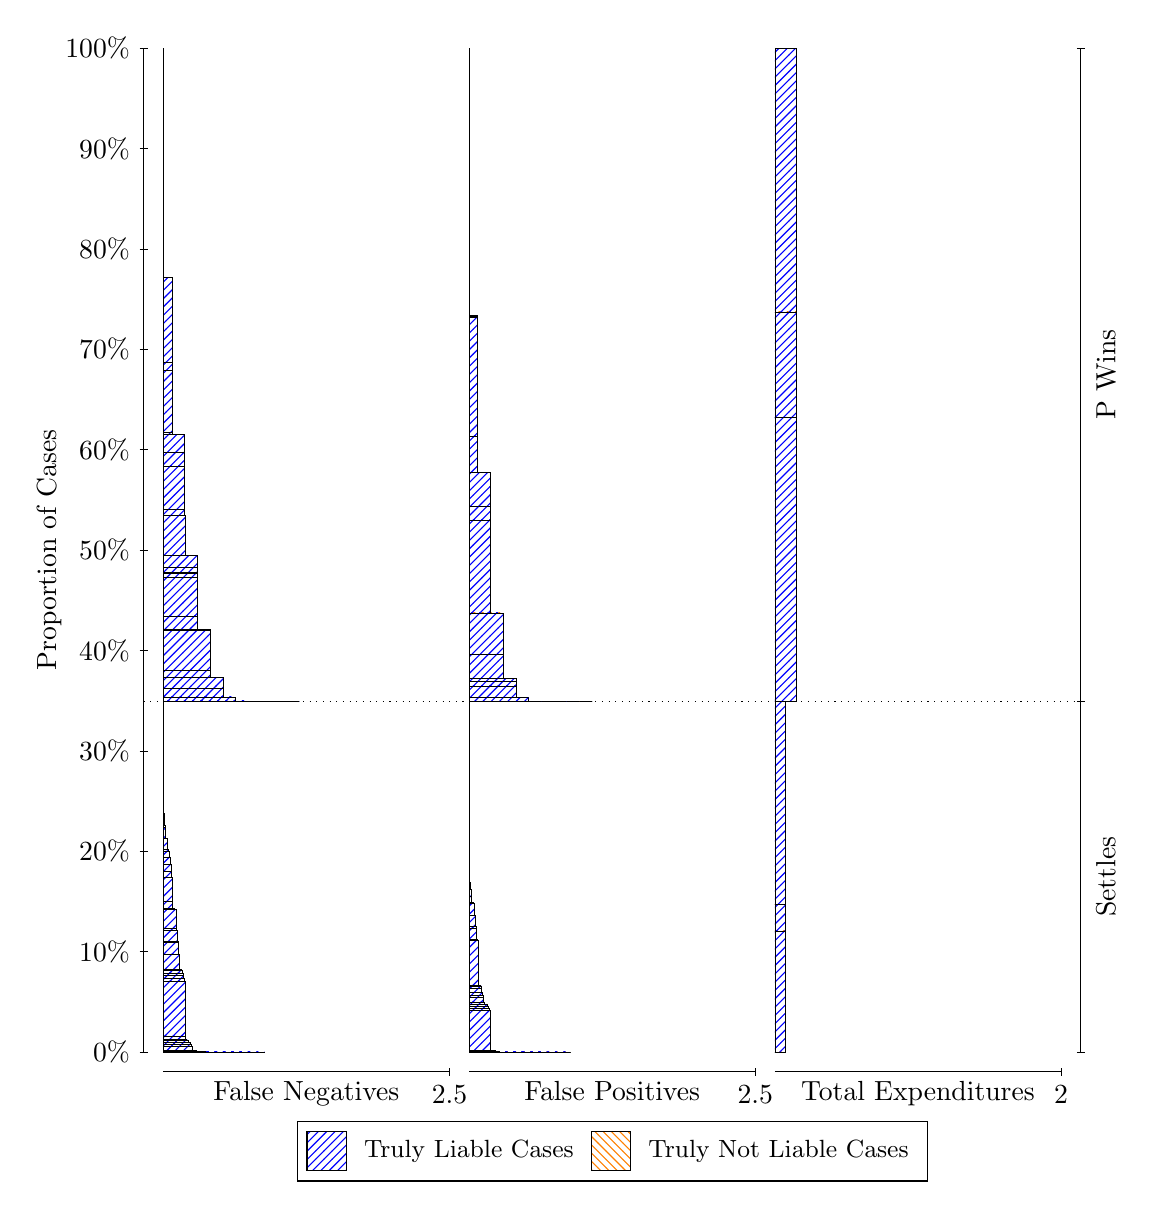
\begin{tikzpicture}
\draw[black, very thin] (1.5,1.75) -- (1.5,14.5);
\node[rotate=90, text=black, anchor=center] at (0.3, 8.125) {Proportion of Cases};
\draw[black, very thin] (1.45,1.75) -- (1.55,1.75);
\node[text=black, anchor=east] at (1.45, 1.75) {0\%};
\draw[black, very thin] (1.45,3.025) -- (1.55,3.025);
\node[text=black, anchor=east] at (1.45, 3.025) {10\%};
\draw[black, very thin] (1.45,4.3) -- (1.55,4.3);
\node[text=black, anchor=east] at (1.45, 4.3) {20\%};
\draw[black, very thin] (1.45,5.575) -- (1.55,5.575);
\node[text=black, anchor=east] at (1.45, 5.575) {30\%};
\draw[black, very thin] (1.45,6.85) -- (1.55,6.85);
\node[text=black, anchor=east] at (1.45, 6.85) {40\%};
\draw[black, very thin] (1.45,8.125) -- (1.55,8.125);
\node[text=black, anchor=east] at (1.45, 8.125) {50\%};
\draw[black, very thin] (1.45,9.4) -- (1.55,9.4);
\node[text=black, anchor=east] at (1.45, 9.4) {60\%};
\draw[black, very thin] (1.45,10.675) -- (1.55,10.675);
\node[text=black, anchor=east] at (1.45, 10.675) {70\%};
\draw[black, very thin] (1.45,11.95) -- (1.55,11.95);
\node[text=black, anchor=east] at (1.45, 11.95) {80\%};
\draw[black, very thin] (1.45,13.225) -- (1.55,13.225);
\node[text=black, anchor=east] at (1.45, 13.225) {90\%};
\draw[black, very thin] (1.45,14.5) -- (1.55,14.5);
\node[text=black, anchor=east] at (1.45, 14.5) {100\%};

\draw[black, very thin] (13.4,1.75) -- (13.4,14.5);
\draw[black, very thin] (13.35,1.75) -- (13.45,1.75);
\node[anchor=west] at (13.35, 1.75) {};
\draw[black, very thin] (13.35,6.2014) -- (13.45,6.2014);
\node[anchor=west] at (13.35, 6.2014) {};
\draw[black, very thin] (13.35,14.5) -- (13.45,14.5);
\node[anchor=west] at (13.35, 14.5) {};

\draw[black, very thin, pattern color=blue, pattern=north east lines] (1.75,1.75) rectangle (3.0398,1.75);
\draw[black, very thin, pattern color=blue, pattern=north east lines] (1.75,1.75) rectangle (2.9672,1.75);
\draw[black, very thin, pattern color=blue, pattern=north east lines] (1.75,1.75) rectangle (2.8945,1.75);
\draw[black, very thin, pattern color=blue, pattern=north east lines] (1.75,1.75) rectangle (2.8784,1.75);
\draw[black, very thin, pattern color=blue, pattern=north east lines] (1.75,1.75) rectangle (2.8218,1.75);
\draw[black, very thin, pattern color=blue, pattern=north east lines] (1.75,1.75) rectangle (2.8057,1.75);
\draw[black, very thin, pattern color=blue, pattern=north east lines] (1.75,1.75) rectangle (2.7492,1.75);
\draw[black, very thin, pattern color=blue, pattern=north east lines] (1.75,1.75) rectangle (2.733,1.75);
\draw[black, very thin, pattern color=blue, pattern=north east lines] (1.75,1.75) rectangle (2.7169,1.75);
\draw[black, very thin, pattern color=blue, pattern=north east lines] (1.75,1.75) rectangle (2.6765,1.75);
\draw[black, very thin, pattern color=blue, pattern=north east lines] (1.75,1.75) rectangle (2.6604,1.75);
\draw[black, very thin, pattern color=blue, pattern=north east lines] (1.75,1.75) rectangle (2.6442,1.75);
\draw[black, very thin, pattern color=blue, pattern=north east lines] (1.75,1.75) rectangle (2.6038,1.75);
\draw[black, very thin, pattern color=blue, pattern=north east lines] (1.75,1.75) rectangle (2.5877,1.75);
\draw[black, very thin, pattern color=blue, pattern=north east lines] (1.75,1.75) rectangle (2.5715,1.75);
\draw[black, very thin, pattern color=blue, pattern=north east lines] (1.75,1.75) rectangle (2.5554,1.75);
\draw[black, very thin, pattern color=blue, pattern=north east lines] (1.75,1.75) rectangle (2.5312,1.75);
\draw[black, very thin, pattern color=blue, pattern=north east lines] (1.75,1.75) rectangle (2.515,1.75);
\draw[black, very thin, pattern color=blue, pattern=north east lines] (1.75,1.75) rectangle (2.4989,1.75);
\draw[black, very thin, pattern color=blue, pattern=north east lines] (1.75,1.75) rectangle (2.4827,1.75);
\draw[black, very thin, pattern color=blue, pattern=north east lines] (1.75,1.75) rectangle (2.4585,1.75);
\draw[black, very thin, pattern color=blue, pattern=north east lines] (1.75,1.75) rectangle (2.4424,1.75);
\draw[black, very thin, pattern color=blue, pattern=north east lines] (1.75,1.75) rectangle (2.4262,1.75);
\draw[black, very thin, pattern color=blue, pattern=north east lines] (1.75,1.75) rectangle (2.4101,1.75);
\draw[black, very thin, pattern color=blue, pattern=north east lines] (1.75,1.75) rectangle (2.3939,1.75);
\draw[black, very thin, pattern color=blue, pattern=north east lines] (1.75,1.75) rectangle (2.3858,1.75);
\draw[black, very thin, pattern color=blue, pattern=north east lines] (1.75,1.75) rectangle (2.3697,1.75);
\draw[black, very thin, pattern color=blue, pattern=north east lines] (1.75,1.75) rectangle (2.3535,1.7501);
\draw[black, very thin, pattern color=blue, pattern=north east lines] (1.75,1.7501) rectangle (2.3374,1.7501);
\draw[black, very thin, pattern color=blue, pattern=north east lines] (1.75,1.7501) rectangle (2.3212,1.7502);
\draw[black, very thin, pattern color=blue, pattern=north east lines] (1.75,1.7502) rectangle (2.3132,1.7502);
\draw[black, very thin, pattern color=blue, pattern=north east lines] (1.75,1.7502) rectangle (2.297,1.7503);
\draw[black, very thin, pattern color=blue, pattern=north east lines] (1.75,1.7503) rectangle (2.2809,1.7526);
\draw[black, very thin, pattern color=blue, pattern=north east lines] (1.75,1.7526) rectangle (2.2647,1.7533);
\draw[black, very thin, pattern color=blue, pattern=north east lines] (1.75,1.7533) rectangle (2.2486,1.7538);
\draw[black, very thin, pattern color=blue, pattern=north east lines] (1.75,1.7538) rectangle (2.2405,1.7539);
\draw[black, very thin, pattern color=blue, pattern=north east lines] (1.75,1.7539) rectangle (2.2324,1.7545);
\draw[black, very thin, pattern color=blue, pattern=north east lines] (1.75,1.7545) rectangle (2.2244,1.7546);
\draw[black, very thin, pattern color=blue, pattern=north east lines] (1.75,1.7546) rectangle (2.2082,1.7547);
\draw[black, very thin, pattern color=blue, pattern=north east lines] (1.75,1.7547) rectangle (2.1921,1.7595);
\draw[black, very thin, pattern color=blue, pattern=north east lines] (1.75,1.7595) rectangle (2.1759,1.7615);
\draw[black, very thin, pattern color=blue, pattern=north east lines] (1.75,1.7615) rectangle (2.1678,1.7656);
\draw[black, very thin, pattern color=blue, pattern=north east lines] (1.75,1.7656) rectangle (2.1598,1.7675);
\draw[black, very thin, pattern color=blue, pattern=north east lines] (1.75,1.7675) rectangle (2.1517,1.7697);
\draw[black, very thin, pattern color=blue, pattern=north east lines] (1.75,1.7697) rectangle (2.1355,1.7727);
\draw[black, very thin, pattern color=blue, pattern=north east lines] (1.75,1.7727) rectangle (2.1194,1.8211);
\draw[black, very thin, pattern color=blue, pattern=north east lines] (1.75,1.8211) rectangle (2.1032,1.8445);
\draw[black, very thin, pattern color=blue, pattern=north east lines] (1.75,1.8445) rectangle (2.0952,1.8506);
\draw[black, very thin, pattern color=blue, pattern=north east lines] (1.75,1.8506) rectangle (2.0871,1.8723);
\draw[black, very thin, pattern color=blue, pattern=north east lines] (1.75,1.8723) rectangle (2.079,1.8757);
\draw[black, very thin, pattern color=blue, pattern=north east lines] (1.75,1.8757) rectangle (2.0709,1.9014);
\draw[black, very thin, pattern color=blue, pattern=north east lines] (1.75,1.9014) rectangle (2.0629,1.9032);
\draw[black, very thin, pattern color=blue, pattern=north east lines] (1.75,1.9032) rectangle (2.0467,1.9051);
\draw[black, very thin, pattern color=blue, pattern=north east lines] (1.75,1.9051) rectangle (2.0306,1.9534);
\draw[black, very thin, pattern color=blue, pattern=north east lines] (1.75,1.9534) rectangle (2.0225,2.6531);
\draw[black, very thin, pattern color=blue, pattern=north east lines] (1.75,2.6531) rectangle (2.0144,2.6851);
\draw[black, very thin, pattern color=blue, pattern=north east lines] (1.75,2.6851) rectangle (2.0064,2.7212);
\draw[black, very thin, pattern color=blue, pattern=north east lines] (1.75,2.7212) rectangle (1.9983,2.7537);
\draw[black, very thin, pattern color=blue, pattern=north east lines] (1.75,2.7537) rectangle (1.9902,2.7841);
\draw[black, very thin, pattern color=blue, pattern=north east lines] (1.75,2.7841) rectangle (1.9741,2.8033);
\draw[black, very thin, pattern color=blue, pattern=north east lines] (1.75,2.8033) rectangle (1.9579,2.9963);
\draw[black, very thin, pattern color=blue, pattern=north east lines] (1.75,2.9963) rectangle (1.9418,3.1377);
\draw[black, very thin, pattern color=blue, pattern=north east lines] (1.75,3.1377) rectangle (1.9337,3.1591);
\draw[black, very thin, pattern color=blue, pattern=north east lines] (1.75,3.1591) rectangle (1.9256,3.2977);
\draw[black, very thin, pattern color=blue, pattern=north east lines] (1.75,3.2977) rectangle (1.9175,3.3166);
\draw[black, very thin, pattern color=blue, pattern=north east lines] (1.75,3.3166) rectangle (1.9095,3.5604);
\draw[black, very thin, pattern color=blue, pattern=north east lines] (1.75,3.5604) rectangle (1.9014,3.5652);
\draw[black, very thin, pattern color=blue, pattern=north east lines] (1.75,3.5652) rectangle (1.8852,3.5699);
\draw[black, very thin, pattern color=blue, pattern=north east lines] (1.75,3.5699) rectangle (1.8691,3.6631);
\draw[black, very thin, pattern color=blue, pattern=north east lines] (1.75,3.6631) rectangle (1.861,3.9698);
\draw[black, very thin, pattern color=blue, pattern=north east lines] (1.75,3.9698) rectangle (1.8529,4.05);
\draw[black, very thin, pattern color=blue, pattern=north east lines] (1.75,4.05) rectangle (1.8449,4.1301);
\draw[black, very thin, pattern color=blue, pattern=north east lines] (1.75,4.1301) rectangle (1.8368,4.2245);
\draw[black, very thin, pattern color=blue, pattern=north east lines] (1.75,4.2245) rectangle (1.8287,4.2995);
\draw[black, very thin, pattern color=blue, pattern=north east lines] (1.75,4.2995) rectangle (1.8126,4.3186);
\draw[black, very thin, pattern color=blue, pattern=north east lines] (1.75,4.3186) rectangle (1.7964,4.4667);
\draw[black, very thin, pattern color=blue, pattern=north east lines] (1.75,4.4667) rectangle (1.7803,4.6053);
\draw[black, very thin, pattern color=blue, pattern=north east lines] (1.75,4.6053) rectangle (1.7722,4.6242);
\draw[black, very thin, pattern color=blue, pattern=north east lines] (1.75,4.6242) rectangle (1.7641,4.7673);
\draw[black, very thin, pattern color=blue, pattern=north east lines] (1.75,4.7673) rectangle (1.7561,4.786);
\draw[black, very thin, pattern color=orange, pattern=north west lines] (1.75,4.786) rectangle (1.75,4.786);
\draw[black, very thin, pattern color=blue, pattern=north east lines] (1.75,4.786) rectangle (1.75,6.2014);
\draw[black, very thin, pattern color=blue, pattern=north east lines] (1.75,6.2014) rectangle (3.4758,6.2014);
\draw[black, very thin, pattern color=blue, pattern=north east lines] (1.75,6.2014) rectangle (3.3144,6.2014);
\draw[black, very thin, pattern color=blue, pattern=north east lines] (1.75,6.2014) rectangle (3.1529,6.2014);
\draw[black, very thin, pattern color=blue, pattern=north east lines] (1.75,6.2014) rectangle (3.1529,6.2014);
\draw[black, very thin, pattern color=blue, pattern=north east lines] (1.75,6.2014) rectangle (3.1509,6.2014);
\draw[black, very thin, pattern color=blue, pattern=north east lines] (1.75,6.2014) rectangle (2.9914,6.2016);
\draw[black, very thin, pattern color=blue, pattern=north east lines] (1.75,6.2016) rectangle (2.9914,6.2019);
\draw[black, very thin, pattern color=blue, pattern=north east lines] (1.75,6.2019) rectangle (2.9894,6.2019);
\draw[black, very thin, pattern color=blue, pattern=north east lines] (1.75,6.2019) rectangle (2.9894,6.2019);
\draw[black, very thin, pattern color=blue, pattern=north east lines] (1.75,6.2019) rectangle (2.8299,6.2082);
\draw[black, very thin, pattern color=blue, pattern=north east lines] (1.75,6.2082) rectangle (2.8279,6.2082);
\draw[black, very thin, pattern color=blue, pattern=north east lines] (1.75,6.2082) rectangle (2.6684,6.2583);
\draw[black, very thin, pattern color=blue, pattern=north east lines] (1.75,6.2583) rectangle (2.6664,6.2583);
\draw[black, very thin, pattern color=blue, pattern=north east lines] (1.75,6.2583) rectangle (2.5069,6.3628);
\draw[black, very thin, pattern color=blue, pattern=north east lines] (1.75,6.3628) rectangle (2.5069,6.5026);
\draw[black, very thin, pattern color=blue, pattern=north east lines] (1.75,6.5026) rectangle (2.5049,6.5026);
\draw[black, very thin, pattern color=blue, pattern=north east lines] (1.75,6.5026) rectangle (2.5049,6.5027);
\draw[black, very thin, pattern color=blue, pattern=north east lines] (1.75,6.5027) rectangle (2.3455,6.5985);
\draw[black, very thin, pattern color=blue, pattern=north east lines] (1.75,6.5985) rectangle (2.3455,7.1084);
\draw[black, very thin, pattern color=blue, pattern=north east lines] (1.75,7.1084) rectangle (2.3434,7.109);
\draw[black, very thin, pattern color=blue, pattern=north east lines] (1.75,7.109) rectangle (2.3434,7.1167);
\draw[black, very thin, pattern color=blue, pattern=north east lines] (1.75,7.1167) rectangle (2.3434,7.1209);
\draw[black, very thin, pattern color=blue, pattern=north east lines] (1.75,7.1209) rectangle (2.184,7.2896);
\draw[black, very thin, pattern color=blue, pattern=north east lines] (1.75,7.2896) rectangle (2.184,7.7803);
\draw[black, very thin, pattern color=blue, pattern=north east lines] (1.75,7.7803) rectangle (2.184,7.8307);
\draw[black, very thin, pattern color=blue, pattern=north east lines] (1.75,7.8307) rectangle (2.182,7.8401);
\draw[black, very thin, pattern color=blue, pattern=north east lines] (1.75,7.8401) rectangle (2.182,7.9057);
\draw[black, very thin, pattern color=blue, pattern=north east lines] (1.75,7.9057) rectangle (2.182,8.0603);
\draw[black, very thin, pattern color=blue, pattern=north east lines] (1.75,8.0603) rectangle (2.0225,8.5627);
\draw[black, very thin, pattern color=blue, pattern=north east lines] (1.75,8.5627) rectangle (2.0205,8.6413);
\draw[black, very thin, pattern color=blue, pattern=north east lines] (1.75,8.6413) rectangle (2.0205,9.1927);
\draw[black, very thin, pattern color=blue, pattern=north east lines] (1.75,9.1927) rectangle (2.0205,9.369);
\draw[black, very thin, pattern color=blue, pattern=north east lines] (1.75,9.369) rectangle (2.0205,9.5957);
\draw[black, very thin, pattern color=blue, pattern=north east lines] (1.75,9.5957) rectangle (1.861,9.5959);
\draw[black, very thin, pattern color=blue, pattern=north east lines] (1.75,9.5959) rectangle (1.861,9.6178);
\draw[black, very thin, pattern color=blue, pattern=north east lines] (1.75,9.6178) rectangle (1.861,9.6179);
\draw[black, very thin, pattern color=blue, pattern=north east lines] (1.75,9.6179) rectangle (1.859,10.405);
\draw[black, very thin, pattern color=blue, pattern=north east lines] (1.75,10.405) rectangle (1.859,10.508);
\draw[black, very thin, pattern color=blue, pattern=north east lines] (1.75,10.508) rectangle (1.859,11.589);
\draw[black, very thin, pattern color=orange, pattern=north west lines] (1.75,11.589) rectangle (1.75,11.589);
\draw[black, very thin, pattern color=blue, pattern=north east lines] (1.75,11.589) rectangle (1.75,14.5);
\draw[black, very thin, pattern color=orange, pattern=north west lines] (5.6333,1.75) rectangle (6.9232,1.75);
\draw[black, very thin, pattern color=blue, pattern=north east lines] (5.6333,1.75) rectangle (6.9232,1.75);
\draw[black, very thin, pattern color=orange, pattern=north west lines] (5.6333,1.75) rectangle (6.8505,1.75);
\draw[black, very thin, pattern color=blue, pattern=north east lines] (5.6333,1.75) rectangle (6.8505,1.75);
\draw[black, very thin, pattern color=orange, pattern=north west lines] (5.6333,1.75) rectangle (6.7778,1.75);
\draw[black, very thin, pattern color=blue, pattern=north east lines] (5.6333,1.75) rectangle (6.7778,1.75);
\draw[black, very thin, pattern color=blue, pattern=north east lines] (5.6333,1.75) rectangle (6.7617,1.75);
\draw[black, very thin, pattern color=orange, pattern=north west lines] (5.6333,1.75) rectangle (6.7052,1.75);
\draw[black, very thin, pattern color=blue, pattern=north east lines] (5.6333,1.75) rectangle (6.7052,1.75);
\draw[black, very thin, pattern color=blue, pattern=north east lines] (5.6333,1.75) rectangle (6.689,1.75);
\draw[black, very thin, pattern color=orange, pattern=north west lines] (5.6333,1.75) rectangle (6.6325,1.75);
\draw[black, very thin, pattern color=blue, pattern=north east lines] (5.6333,1.75) rectangle (6.6325,1.75);
\draw[black, very thin, pattern color=blue, pattern=north east lines] (5.6333,1.75) rectangle (6.6164,1.75);
\draw[black, very thin, pattern color=blue, pattern=north east lines] (5.6333,1.75) rectangle (6.6002,1.75);
\draw[black, very thin, pattern color=orange, pattern=north west lines] (5.6333,1.75) rectangle (6.5598,1.75);
\draw[black, very thin, pattern color=blue, pattern=north east lines] (5.6333,1.75) rectangle (6.5598,1.75);
\draw[black, very thin, pattern color=blue, pattern=north east lines] (5.6333,1.75) rectangle (6.5437,1.75);
\draw[black, very thin, pattern color=blue, pattern=north east lines] (5.6333,1.75) rectangle (6.5275,1.75);
\draw[black, very thin, pattern color=orange, pattern=north west lines] (5.6333,1.75) rectangle (6.4872,1.75);
\draw[black, very thin, pattern color=blue, pattern=north east lines] (5.6333,1.75) rectangle (6.4872,1.75);
\draw[black, very thin, pattern color=blue, pattern=north east lines] (5.6333,1.75) rectangle (6.471,1.75);
\draw[black, very thin, pattern color=blue, pattern=north east lines] (5.6333,1.75) rectangle (6.4549,1.75);
\draw[black, very thin, pattern color=blue, pattern=north east lines] (5.6333,1.75) rectangle (6.4387,1.75);
\draw[black, very thin, pattern color=orange, pattern=north west lines] (5.6333,1.75) rectangle (6.4145,1.75);
\draw[black, very thin, pattern color=blue, pattern=north east lines] (5.6333,1.75) rectangle (6.4145,1.75);
\draw[black, very thin, pattern color=blue, pattern=north east lines] (5.6333,1.75) rectangle (6.3984,1.75);
\draw[black, very thin, pattern color=blue, pattern=north east lines] (5.6333,1.75) rectangle (6.3822,1.75);
\draw[black, very thin, pattern color=blue, pattern=north east lines] (5.6333,1.75) rectangle (6.3661,1.75);
\draw[black, very thin, pattern color=orange, pattern=north west lines] (5.6333,1.75) rectangle (6.3418,1.75);
\draw[black, very thin, pattern color=blue, pattern=north east lines] (5.6333,1.75) rectangle (6.3418,1.75);
\draw[black, very thin, pattern color=blue, pattern=north east lines] (5.6333,1.75) rectangle (6.3257,1.75);
\draw[black, very thin, pattern color=blue, pattern=north east lines] (5.6333,1.75) rectangle (6.3095,1.75);
\draw[black, very thin, pattern color=blue, pattern=north east lines] (5.6333,1.75) rectangle (6.2934,1.75);
\draw[black, very thin, pattern color=blue, pattern=north east lines] (5.6333,1.75) rectangle (6.2772,1.75);
\draw[black, very thin, pattern color=orange, pattern=north west lines] (5.6333,1.75) rectangle (6.2692,1.75);
\draw[black, very thin, pattern color=blue, pattern=north east lines] (5.6333,1.75) rectangle (6.2692,1.75);
\draw[black, very thin, pattern color=blue, pattern=north east lines] (5.6333,1.75) rectangle (6.253,1.75);
\draw[black, very thin, pattern color=blue, pattern=north east lines] (5.6333,1.75) rectangle (6.2369,1.75);
\draw[black, very thin, pattern color=blue, pattern=north east lines] (5.6333,1.75) rectangle (6.2207,1.75);
\draw[black, very thin, pattern color=blue, pattern=north east lines] (5.6333,1.75) rectangle (6.2046,1.75);
\draw[black, very thin, pattern color=orange, pattern=north west lines] (5.6333,1.75) rectangle (6.1965,1.75);
\draw[black, very thin, pattern color=blue, pattern=north east lines] (5.6333,1.75) rectangle (6.1965,1.75);
\draw[black, very thin, pattern color=blue, pattern=north east lines] (5.6333,1.75) rectangle (6.1804,1.75);
\draw[black, very thin, pattern color=blue, pattern=north east lines] (5.6333,1.75) rectangle (6.1642,1.75);
\draw[black, very thin, pattern color=blue, pattern=north east lines] (5.6333,1.75) rectangle (6.1481,1.75);
\draw[black, very thin, pattern color=blue, pattern=north east lines] (5.6333,1.75) rectangle (6.1319,1.75);
\draw[black, very thin, pattern color=orange, pattern=north west lines] (5.6333,1.75) rectangle (6.1238,1.75);
\draw[black, very thin, pattern color=blue, pattern=north east lines] (5.6333,1.75) rectangle (6.1238,1.7501);
\draw[black, very thin, pattern color=blue, pattern=north east lines] (5.6333,1.7501) rectangle (6.1158,1.7501);
\draw[black, very thin, pattern color=blue, pattern=north east lines] (5.6333,1.7501) rectangle (6.1077,1.7501);
\draw[black, very thin, pattern color=blue, pattern=north east lines] (5.6333,1.7501) rectangle (6.0915,1.7501);
\draw[black, very thin, pattern color=blue, pattern=north east lines] (5.6333,1.7501) rectangle (6.0754,1.7501);
\draw[black, very thin, pattern color=blue, pattern=north east lines] (5.6333,1.7501) rectangle (6.0592,1.7502);
\draw[black, very thin, pattern color=orange, pattern=north west lines] (5.6333,1.7502) rectangle (6.0512,1.7502);
\draw[black, very thin, pattern color=blue, pattern=north east lines] (5.6333,1.7502) rectangle (6.0512,1.7515);
\draw[black, very thin, pattern color=blue, pattern=north east lines] (5.6333,1.7515) rectangle (6.0431,1.7516);
\draw[black, very thin, pattern color=blue, pattern=north east lines] (5.6333,1.7516) rectangle (6.035,1.7522);
\draw[black, very thin, pattern color=blue, pattern=north east lines] (5.6333,1.7522) rectangle (6.0189,1.7527);
\draw[black, very thin, pattern color=blue, pattern=north east lines] (5.6333,1.7527) rectangle (6.0027,1.7528);
\draw[black, very thin, pattern color=blue, pattern=north east lines] (5.6333,1.7528) rectangle (5.9866,1.7546);
\draw[black, very thin, pattern color=orange, pattern=north west lines] (5.6333,1.7546) rectangle (5.9785,1.7546);
\draw[black, very thin, pattern color=blue, pattern=north east lines] (5.6333,1.7546) rectangle (5.9785,1.7646);
\draw[black, very thin, pattern color=blue, pattern=north east lines] (5.6333,1.7646) rectangle (5.9704,1.7665);
\draw[black, very thin, pattern color=blue, pattern=north east lines] (5.6333,1.7665) rectangle (5.9624,1.7689);
\draw[black, very thin, pattern color=blue, pattern=north east lines] (5.6333,1.7689) rectangle (5.9543,1.7712);
\draw[black, very thin, pattern color=blue, pattern=north east lines] (5.6333,1.7712) rectangle (5.9462,1.7732);
\draw[black, very thin, pattern color=blue, pattern=north east lines] (5.6333,1.7732) rectangle (5.9301,1.7733);
\draw[black, very thin, pattern color=blue, pattern=north east lines] (5.6333,1.7733) rectangle (5.9139,1.7734);
\draw[black, very thin, pattern color=orange, pattern=north west lines] (5.6333,1.7734) rectangle (5.9058,1.7734);
\draw[black, very thin, pattern color=blue, pattern=north east lines] (5.6333,1.7734) rectangle (5.9058,2.277);
\draw[black, very thin, pattern color=blue, pattern=north east lines] (5.6333,2.277) rectangle (5.8978,2.2799);
\draw[black, very thin, pattern color=blue, pattern=north east lines] (5.6333,2.2799) rectangle (5.8897,2.3068);
\draw[black, very thin, pattern color=blue, pattern=north east lines] (5.6333,2.3068) rectangle (5.8816,2.3097);
\draw[black, very thin, pattern color=blue, pattern=north east lines] (5.6333,2.3097) rectangle (5.8735,2.3317);
\draw[black, very thin, pattern color=blue, pattern=north east lines] (5.6333,2.3317) rectangle (5.8574,2.3523);
\draw[black, very thin, pattern color=blue, pattern=north east lines] (5.6333,2.3523) rectangle (5.8412,2.3553);
\draw[black, very thin, pattern color=blue, pattern=north east lines] (5.6333,2.3553) rectangle (5.8251,2.385);
\draw[black, very thin, pattern color=blue, pattern=north east lines] (5.6333,2.385) rectangle (5.817,2.4404);
\draw[black, very thin, pattern color=blue, pattern=north east lines] (5.6333,2.4404) rectangle (5.8089,2.4718);
\draw[black, very thin, pattern color=blue, pattern=north east lines] (5.6333,2.4718) rectangle (5.8009,2.5042);
\draw[black, very thin, pattern color=blue, pattern=north east lines] (5.6333,2.5042) rectangle (5.7928,2.5578);
\draw[black, very thin, pattern color=blue, pattern=north east lines] (5.6333,2.5578) rectangle (5.7847,2.5903);
\draw[black, very thin, pattern color=blue, pattern=north east lines] (5.6333,2.5903) rectangle (5.7686,2.5922);
\draw[black, very thin, pattern color=blue, pattern=north east lines] (5.6333,2.5922) rectangle (5.7524,2.5941);
\draw[black, very thin, pattern color=blue, pattern=north east lines] (5.6333,2.5941) rectangle (5.7444,3.1654);
\draw[black, very thin, pattern color=blue, pattern=north east lines] (5.6333,3.1654) rectangle (5.7363,3.184);
\draw[black, very thin, pattern color=blue, pattern=north east lines] (5.6333,3.184) rectangle (5.7282,3.3272);
\draw[black, very thin, pattern color=blue, pattern=north east lines] (5.6333,3.3272) rectangle (5.7201,3.3461);
\draw[black, very thin, pattern color=blue, pattern=north east lines] (5.6333,3.3461) rectangle (5.7121,3.4847);
\draw[black, very thin, pattern color=blue, pattern=north east lines] (5.6333,3.4847) rectangle (5.6959,3.6328);
\draw[black, very thin, pattern color=blue, pattern=north east lines] (5.6333,3.6328) rectangle (5.6798,3.6519);
\draw[black, very thin, pattern color=blue, pattern=north east lines] (5.6333,3.6519) rectangle (5.6636,3.7269);
\draw[black, very thin, pattern color=blue, pattern=north east lines] (5.6333,3.7269) rectangle (5.6555,3.8213);
\draw[black, very thin, pattern color=blue, pattern=north east lines] (5.6333,3.8213) rectangle (5.6475,3.9014);
\draw[black, very thin, pattern color=blue, pattern=north east lines] (5.6333,3.9014) rectangle (5.6394,3.9816);
\draw[black, very thin, pattern color=blue, pattern=north east lines] (5.6333,3.9816) rectangle (5.6333,6.2014);
\draw[black, very thin, pattern color=orange, pattern=north west lines] (5.6333,6.2014) rectangle (7.1957,6.2014);
\draw[black, very thin, pattern color=blue, pattern=north east lines] (5.6333,6.2014) rectangle (7.1957,6.2014);
\draw[black, very thin, pattern color=orange, pattern=north west lines] (5.6333,6.2014) rectangle (7.0342,6.2014);
\draw[black, very thin, pattern color=blue, pattern=north east lines] (5.6333,6.2014) rectangle (7.0342,6.2014);
\draw[black, very thin, pattern color=orange, pattern=north west lines] (5.6333,6.2014) rectangle (6.8727,6.2014);
\draw[black, very thin, pattern color=blue, pattern=north east lines] (5.6333,6.2014) rectangle (6.8727,6.2014);
\draw[black, very thin, pattern color=blue, pattern=north east lines] (5.6333,6.2014) rectangle (6.8727,6.2014);
\draw[black, very thin, pattern color=blue, pattern=north east lines] (5.6333,6.2014) rectangle (6.7112,6.2016);
\draw[black, very thin, pattern color=orange, pattern=north west lines] (5.6333,6.2016) rectangle (6.7112,6.2016);
\draw[black, very thin, pattern color=blue, pattern=north east lines] (5.6333,6.2016) rectangle (6.7112,6.2018);
\draw[black, very thin, pattern color=orange, pattern=north west lines] (5.6333,6.2018) rectangle (6.5497,6.2018);
\draw[black, very thin, pattern color=blue, pattern=north east lines] (5.6333,6.2018) rectangle (6.5497,6.2072);
\draw[black, very thin, pattern color=orange, pattern=north west lines] (5.6333,6.2072) rectangle (6.5477,6.2072);
\draw[black, very thin, pattern color=blue, pattern=north east lines] (5.6333,6.2072) rectangle (6.5477,6.2072);
\draw[black, very thin, pattern color=orange, pattern=north west lines] (5.6333,6.2072) rectangle (6.3883,6.2072);
\draw[black, very thin, pattern color=blue, pattern=north east lines] (5.6333,6.2072) rectangle (6.3883,6.2521);
\draw[black, very thin, pattern color=orange, pattern=north west lines] (5.6333,6.2521) rectangle (6.3862,6.2521);
\draw[black, very thin, pattern color=blue, pattern=north east lines] (5.6333,6.2521) rectangle (6.3862,6.2521);
\draw[black, very thin, pattern color=blue, pattern=north east lines] (5.6333,6.2521) rectangle (6.3862,6.2521);
\draw[black, very thin, pattern color=orange, pattern=north west lines] (5.6333,6.2521) rectangle (6.2268,6.2521);
\draw[black, very thin, pattern color=blue, pattern=north east lines] (5.6333,6.2521) rectangle (6.2268,6.3996);
\draw[black, very thin, pattern color=blue, pattern=north east lines] (5.6333,6.3996) rectangle (6.2268,6.4585);
\draw[black, very thin, pattern color=blue, pattern=north east lines] (5.6333,6.4585) rectangle (6.2268,6.4945);
\draw[black, very thin, pattern color=blue, pattern=north east lines] (5.6333,6.4945) rectangle (6.2248,6.4945);
\draw[black, very thin, pattern color=orange, pattern=north west lines] (5.6333,6.4945) rectangle (6.2248,6.4945);
\draw[black, very thin, pattern color=blue, pattern=north east lines] (5.6333,6.4945) rectangle (6.2248,6.4945);
\draw[black, very thin, pattern color=orange, pattern=north west lines] (5.6333,6.4945) rectangle (6.0653,6.4945);
\draw[black, very thin, pattern color=blue, pattern=north east lines] (5.6333,6.4945) rectangle (6.0653,6.7998);
\draw[black, very thin, pattern color=blue, pattern=north east lines] (5.6333,6.7998) rectangle (6.0653,7.3262);
\draw[black, very thin, pattern color=blue, pattern=north east lines] (5.6333,7.3262) rectangle (6.0633,7.3262);
\draw[black, very thin, pattern color=orange, pattern=north west lines] (5.6333,7.3262) rectangle (6.0633,7.3262);
\draw[black, very thin, pattern color=blue, pattern=north east lines] (5.6333,7.3262) rectangle (6.0633,7.3262);
\draw[black, very thin, pattern color=orange, pattern=north west lines] (5.6333,7.3262) rectangle (5.9038,7.3262);
\draw[black, very thin, pattern color=blue, pattern=north east lines] (5.6333,7.3262) rectangle (5.9038,8.5061);
\draw[black, very thin, pattern color=blue, pattern=north east lines] (5.6333,8.5061) rectangle (5.9038,8.6764);
\draw[black, very thin, pattern color=blue, pattern=north east lines] (5.6333,8.6764) rectangle (5.9038,9.1122);
\draw[black, very thin, pattern color=blue, pattern=north east lines] (5.6333,9.1122) rectangle (5.9018,9.1122);
\draw[black, very thin, pattern color=orange, pattern=north west lines] (5.6333,9.1122) rectangle (5.9018,9.1122);
\draw[black, very thin, pattern color=blue, pattern=north east lines] (5.6333,9.1122) rectangle (5.9018,9.1122);
\draw[black, very thin, pattern color=blue, pattern=north east lines] (5.6333,9.1122) rectangle (5.7423,9.5749);
\draw[black, very thin, pattern color=blue, pattern=north east lines] (5.6333,9.5749) rectangle (5.7423,11.084);
\draw[black, very thin, pattern color=blue, pattern=north east lines] (5.6333,11.084) rectangle (5.7403,11.084);
\draw[black, very thin, pattern color=blue, pattern=north east lines] (5.6333,11.084) rectangle (5.7403,11.087);
\draw[black, very thin, pattern color=orange, pattern=north west lines] (5.6333,11.087) rectangle (5.7403,11.087);
\draw[black, very thin, pattern color=blue, pattern=north east lines] (5.6333,11.087) rectangle (5.7403,11.106);
\draw[black, very thin, pattern color=blue, pattern=north east lines] (5.6333,11.106) rectangle (5.7403,11.106);
\draw[black, very thin, pattern color=orange, pattern=north west lines] (5.6333,11.106) rectangle (5.6333,11.106);
\draw[black, very thin, pattern color=blue, pattern=north east lines] (5.6333,11.106) rectangle (5.6333,14.5);
\draw[black, very thin, pattern color=orange, pattern=north west lines] (9.5167,1.75) rectangle (9.6529,1.75);
\draw[black, very thin, pattern color=blue, pattern=north east lines] (9.5167,1.75) rectangle (9.6529,3.2891);
\draw[black, very thin, pattern color=orange, pattern=north west lines] (9.5167,3.2891) rectangle (9.6529,3.2891);
\draw[black, very thin, pattern color=blue, pattern=north east lines] (9.5167,3.2891) rectangle (9.6529,3.6213);
\draw[black, very thin, pattern color=orange, pattern=north west lines] (9.5167,3.6213) rectangle (9.6529,3.6213);
\draw[black, very thin, pattern color=blue, pattern=north east lines] (9.5167,3.6213) rectangle (9.6529,6.2014);
\draw[black, very thin, pattern color=orange, pattern=north west lines] (9.5167,6.2014) rectangle (9.7892,6.2014);
\draw[black, very thin, pattern color=blue, pattern=north east lines] (9.5167,6.2014) rectangle (9.7892,9.8121);
\draw[black, very thin, pattern color=orange, pattern=north west lines] (9.5167,9.8121) rectangle (9.7892,9.8121);
\draw[black, very thin, pattern color=blue, pattern=north east lines] (9.5167,9.8121) rectangle (9.7892,11.15);
\draw[black, very thin, pattern color=orange, pattern=north west lines] (9.5167,11.15) rectangle (9.7892,11.15);
\draw[black, very thin, pattern color=blue, pattern=north east lines] (9.5167,11.15) rectangle (9.7892,14.5);
\draw[black, dotted] (1.5,6.2014) -- (13.4,6.2014);
\draw[black, very thin] (1.75,1.5) -- (5.3833,1.5);
\node[text=black, anchor=north] at (3.5667, 1.5) {False Negatives};
\draw[black, very thin] (5.3833,1.45) -- (5.3833,1.55);
\node[text=black, anchor=north] at (5.3833, 1.45) {2.5};

\draw[black, very thin] (5.6333,1.5) -- (9.2667,1.5);
\node[text=black, anchor=north] at (7.45, 1.5) {False Positives};
\draw[black, very thin] (9.2667,1.45) -- (9.2667,1.55);
\node[text=black, anchor=north] at (9.2667, 1.45) {2.5};

\draw[black, very thin] (9.5167,1.5) -- (13.15,1.5);
\node[text=black, anchor=north] at (11.333, 1.5) {Total Expenditures};
\draw[black, very thin] (13.15,1.45) -- (13.15,1.55);
\node[text=black, anchor=north] at (13.15, 1.45) {2};

\node[text=black, centered, rotate=90] at (13.72, 3.9757) {Settles};
\node[text=black, centered, rotate=90] at (13.72, 10.351) {P Wins};

\draw (7.449999999999999,1.5) node[draw=none] (baseCoordinate) {};
\begin{scope}[align=center]
        \matrix[scale=0.5, draw=black, below=0.5cm of baseCoordinate, nodes={draw}, column sep=0.1cm]{
            \node[rectangle, draw, minimum width=0.5cm, minimum height=0.5cm, pattern color=blue, pattern=north east lines] {}; &
            \node[draw=none, font=\small, text=black] (B) {Truly Liable Cases}; &
            \node[rectangle, draw, minimum width=0.5cm, minimum height=0.5cm, pattern color=orange, pattern=north west lines] {}; &
            \node[draw=none, font=\small, text=black] (B) {Truly Not Liable Cases}; \\
            };
\end{scope}

\end{tikzpicture}
\end{document}